\documentclass[11pt,a4paper]{article}
\usepackage{tikz}
\usetikzlibrary{chains,positioning,calc,shapes.geometric}
\tikzset{flowItem/.style={rectangle,rounded corners,text centered,draw=gray,very thick, on chain},decisionItem/.style={diamond,rounded corners,text centered,draw=gray,very thick, on chain}}
\begin{document}
	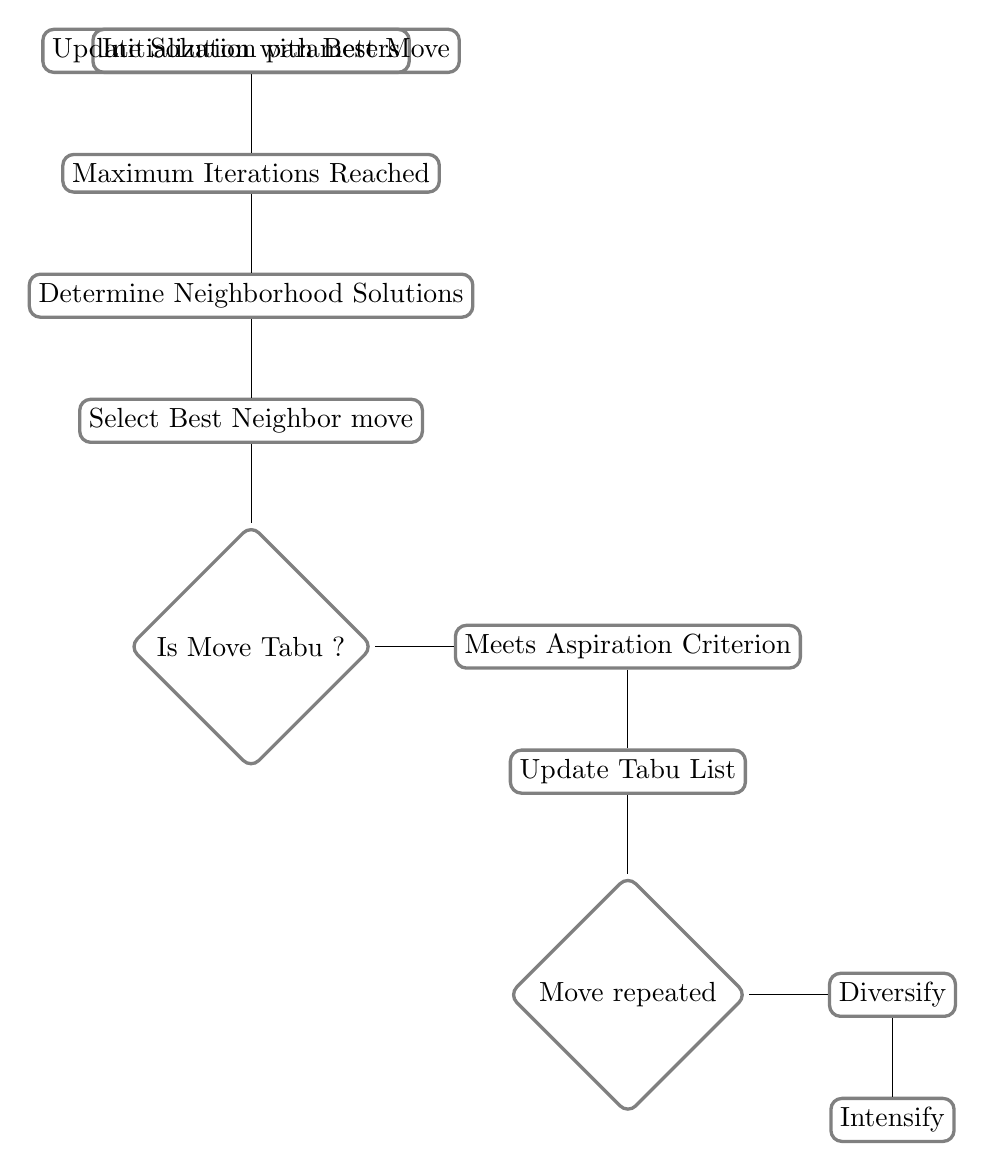
\begin{tikzpicture}[start chain=main going below]
		\node [flowItem,join] {Initialization parameters};
		\node [flowItem,join] {Maximum Iterations Reached};
		\node [flowItem,join] {Determine Neighborhood Solutions};
		\node [flowItem,join] {Select Best Neighbor move};
		\begin{scope}
		\node [decisionItem,join] {Is Move Tabu ?};
		{
			[start branch=Tabu]
			\node [rectangle,rounded corners,text centered, draw=gray,very thick,on chain=going right, join] {Meets Aspiration Criterion};
		}
		\end{scope}
		\node [rectangle,rounded corners,text centered, draw=gray,very thick,continue chain=main, join] {Update Solution with Best Move};
		\node [rectangle,rounded corners,text centered, draw=gray,very thick,on chain=main, join] {Update Tabu List};
		\node [diamond,rounded corners,text centered,draw=gray,very thick, on chain=main,join] {Move repeated};
		{
			[start branch=MoveRepeat]
			\node [rectangle,rounded corners,text centered, draw=gray,very thick,on chain=going right, join] {Diversify};
		}
		\node [rectangle,rounded corners,text centered, draw=gray,very thick,on chain=main, join] {Intensify};
		%Tabu search for global optimization of continuous functions with application to phase equilibrium calculations
		%Tabu Search directed by direct search methods for nonlinear global optimization
		%A tabu search heuristic for the component assignment problem in PCB assembly
		%A Tabu Search Approach for the Single Machine Mean Tardiness Problem
		%Tabu Search applied to global optimization
		%Multiple Sequence Alignment Using Tabu Search
	\end{tikzpicture}
\end{document}
